\documentclass{article}
\usepackage{graphicx}
\usepackage{hyperref}
\title{Reproducing the Correlation Function of Halos at $z=3$}
\author{Felipe G\'omez-Cort\'es}


\begin{document}
 
 \maketitle 
 \bibliographystyle{plain}
 
 \section{Introduction}
 The first goal is to reproduce the halo correlation function at $z=3$ in the 
 Conroy et. al. (2006)\cite{Conroy06} paper (figure 4). The number density of halos
 in this paper is $n=1.5\times10^{-2}h^3 \textrm{Mpc}^{-3}$.

  \begin{equation}
  \omega_p(r_p) = 2 \int_0^\infty \xi \left( \sqrt{r_p^2 + r_\parallel^2} \right) dr_\parallel
 \end{equation}

 
 \section{Dark Matter Halo Catalog}
 
 The DM halo catalog was retreived from the BolshoiP Simulation.\footnote{Available at 
 \url{https://www.cosmosim.org/cms/simulations/bolshoip-project/bolshoip/}}
 This is contained in a cubic box of lenght $L = 250 \textrm{Mpc }h^{-1}$,  
 The halos where choosen form the BDM\footnote{Bound Density
 Maximum $\Delta = 360\rho_\textrm{background}$} catalog in the snapshot 87 ($z=2.952$).
 
   
 \section{Correlation Function using AstroML library}
 The astroML Library uses a \textit{k-d Tree method}. This is a extremly efficient method
 to calculate correlation functions.  With a 230.000 points catalog, the brute force 
 method takes around 84.000 seconds to  find the correlation function, while the k-d 
 tree method takes only 27 seconds.
 
 There is only one issue with the code: the normalization factor seems to be corrected
 by the boxlenght $L$.
 
 Installation using Conda on Mac, or in Linux:
 \begin{verbatim}
 sudo pip install scipy
 sudo pip install astropy
 sudo pip install astroML
 sudo pip install astroML_addons
 sudo pip install scikit-learn
 \end{verbatim}
 
 
 
 \begin{figure}
 \begin{center}
  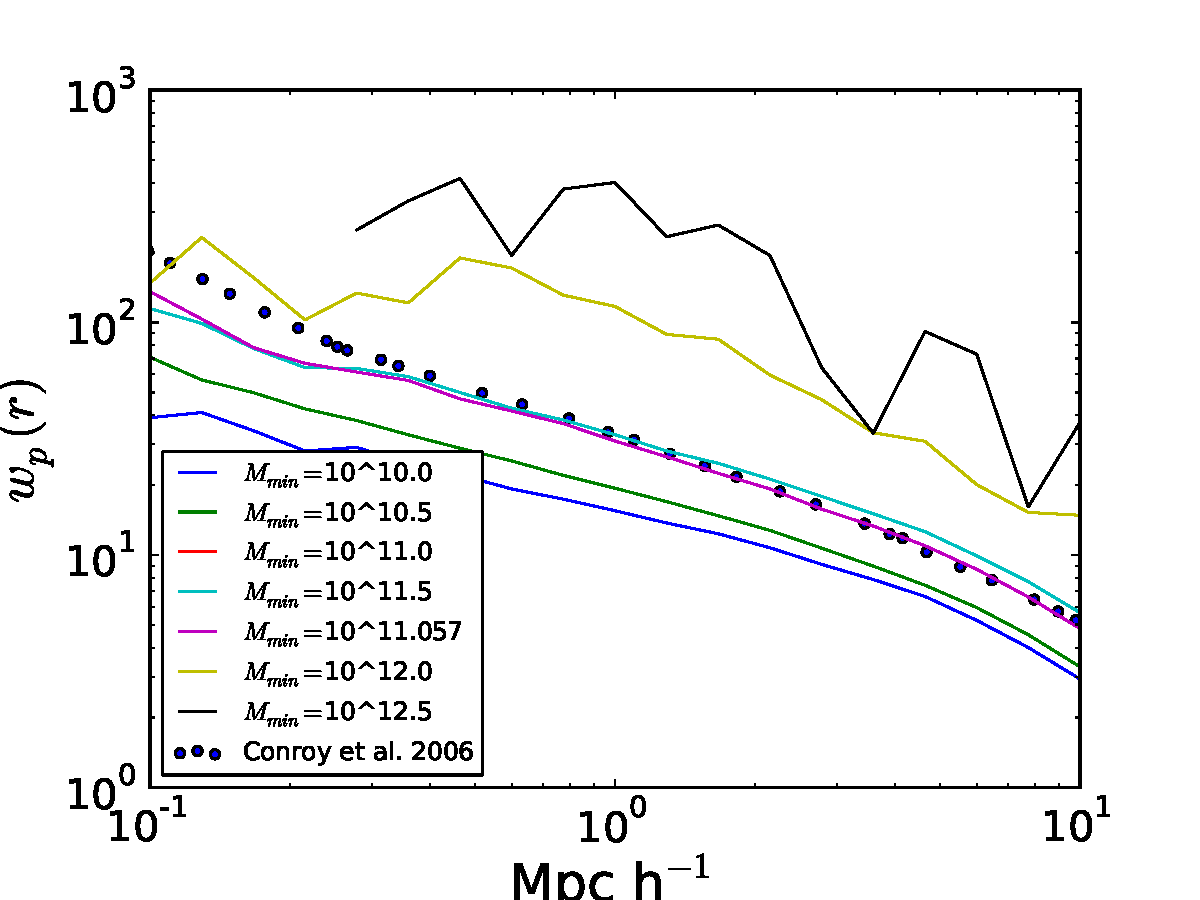
\includegraphics[height=7.0cm]{projected_correlation_astroML00.pdf}
  \caption{Halo Projected Correlation Function with different cuttoff masses.
  $\log_{10}(M_\textrm{halo}/M_\odot) = 10.0, 10.5, 11.0, 11.5, 11.057, 12.0 \and 12.5$}
 \end{center}
 \end{figure}

  
 \bibliography{report}

 
 
 
\end{document}

